% =====================================================================
% From Flat to Micro-Segmented: A Simulation-Based Evaluation of
% Lateral-Movement Containment for Compromised IoMT Devices in a
% Smart-Hospital Network
%
% Format: IEEE conference template conference_101719.tex
% (IEEE_Conference_Template__1_.zip in the project root; its IEEEtran.cls
% is byte-identical to the copy in this folder, see README.md).
% Build: powershell -ExecutionPolicy Bypass -File build.ps1
%   (regenerates tables/ and figures/ from ../results and ../configs,
%    then compiles if LaTeX is present, otherwise writes overleaf.zip)
% =====================================================================
\documentclass[conference]{IEEEtran}
\IEEEoverridecommandlockouts
% The preceding line is only needed to identify funding in the first footnote. If that is unneeded, please comment it out.

% ---- packages of the IEEE conference template ----
\usepackage{cite}
\usepackage{amsmath,amssymb,amsfonts}
\usepackage{algorithmic}
\usepackage{graphicx}
\usepackage{textcomp}
\usepackage{xcolor}
% ---- additions this paper needs ----
\usepackage[T1]{fontenc}  % hyphenation of words with accents; Times stays the body font
\usepackage{booktabs}     % \toprule/\midrule/\bottomrule in the generated tables
\usepackage{url}          % URLs in the references
\usepackage{balance}      % equal columns on the last page

\graphicspath{{figures/}}

% ---- outcome symbols used by the generated tables (robust: used in captions) ----
\DeclareRobustCommand{\outcomebox}[2]{{\setlength{\fboxsep}{1.2pt}\colorbox{#1}{\makebox[1.1em]{\textbf{#2}}}}}
\DeclareRobustCommand{\oS}{\outcomebox{red!30}{S}}      % attack succeeded
\DeclareRobustCommand{\oP}{\outcomebox{yellow!45}{P}}   % partial: some targets reachable
\DeclareRobustCommand{\oB}{\outcomebox{green!25}{B}}    % blocked
\DeclareRobustCommand{\cmark}{\ensuremath{\checkmark}}
\DeclareRobustCommand{\xmark}{\ensuremath{\times}}

% ---- data switches and numbers written by gen_tables.py ----
\newif\ifmeasured       % true only when every observed column of the core tests is filled
\newif\ifhavestatic     % results/static-analysis*.csv present
\newif\ifhavefix        % paper/data/fix-impact.csv present
\newif\ifhavemetrics    % results/metrics.csv present
\newif\ifhaveoverhead   % results/overhead.csv has measured values
\newif\ifhavedetection  % results/detection.csv present
\newif\ifhaveqone       % Q1 timings measured
% AUTO-GENERATED by paper/gen_tables.py -- do not edit by hand; edit the data and re-run.
% Numbers used in the prose. Regenerated with the tables so text and tables agree.
\providecommand{\cfgLinesDzero}{}\renewcommand{\cfgLinesDzero}{189}
\providecommand{\acesDzero}{}\renewcommand{\acesDzero}{1}
\providecommand{\featDzero}{}\renewcommand{\featDzero}{0}
\providecommand{\devsDzero}{}\renewcommand{\devsDzero}{7}
\providecommand{\cfgLinesDone}{}\renewcommand{\cfgLinesDone}{274}
\providecommand{\acesDone}{}\renewcommand{\acesDone}{1}
\providecommand{\featDone}{}\renewcommand{\featDone}{1}
\providecommand{\devsDone}{}\renewcommand{\devsDone}{7}
\providecommand{\cfgLinesDtwo}{}\renewcommand{\cfgLinesDtwo}{302}
\providecommand{\acesDtwo}{}\renewcommand{\acesDtwo}{17}
\providecommand{\featDtwo}{}\renewcommand{\featDtwo}{2}
\providecommand{\devsDtwo}{}\renewcommand{\devsDtwo}{7}
\providecommand{\cfgLinesDthree}{}\renewcommand{\cfgLinesDthree}{571}
\providecommand{\acesDthree}{}\renewcommand{\acesDthree}{52}
\providecommand{\featDthree}{}\renewcommand{\featDthree}{12}
\providecommand{\devsDthree}{}\renewcommand{\devsDthree}{8}
\providecommand{\deltaLinesDone}{}\renewcommand{\deltaLinesDone}{85}
\providecommand{\deltaAcesDone}{}\renewcommand{\deltaAcesDone}{0}
\providecommand{\deltaLinesDtwo}{}\renewcommand{\deltaLinesDtwo}{28}
\providecommand{\deltaAcesDtwo}{}\renewcommand{\deltaAcesDtwo}{16}
\providecommand{\deltaLinesDthree}{}\renewcommand{\deltaLinesDthree}{269}
\providecommand{\deltaAcesDthree}{}\renewcommand{\deltaAcesDthree}{35}
\providecommand{\lineRatioDthree}{}\renewcommand{\lineRatioDthree}{3.02}
\providecommand{\featListDthree}{}\renewcommand{\featListDthree}{VLAN segmentation, Inter-VLAN ACLs, Stateful firewall (ASA), Port security, DHCP snooping, SSH-only management, VTY source restriction, BPDU Guard / PortFast, Native-VLAN hardening, Trunk allowed-VLAN pruning, Unused ports disabled, Password encryption}
\providecommand{\aceAsaDzero}{}\renewcommand{\aceAsaDzero}{0}
\providecommand{\aceCoreDzero}{}\renewcommand{\aceCoreDzero}{0}
\providecommand{\aceStdDzero}{}\renewcommand{\aceStdDzero}{1}
\providecommand{\aceTotalDzero}{}\renewcommand{\aceTotalDzero}{1}
\providecommand{\aceAsaDone}{}\renewcommand{\aceAsaDone}{0}
\providecommand{\aceCoreDone}{}\renewcommand{\aceCoreDone}{0}
\providecommand{\aceStdDone}{}\renewcommand{\aceStdDone}{1}
\providecommand{\aceTotalDone}{}\renewcommand{\aceTotalDone}{1}
\providecommand{\aceAsaDtwo}{}\renewcommand{\aceAsaDtwo}{0}
\providecommand{\aceCoreDtwo}{}\renewcommand{\aceCoreDtwo}{16}
\providecommand{\aceStdDtwo}{}\renewcommand{\aceStdDtwo}{1}
\providecommand{\aceTotalDtwo}{}\renewcommand{\aceTotalDtwo}{17}
\providecommand{\aceAsaDthree}{}\renewcommand{\aceAsaDthree}{16}
\providecommand{\aceCoreDthree}{}\renewcommand{\aceCoreDthree}{30}
\providecommand{\aceStdDthree}{}\renewcommand{\aceStdDthree}{6}
\providecommand{\aceTotalDthree}{}\renewcommand{\aceTotalDthree}{52}
\providecommand{\attackStatus}{}\renewcommand{\attackStatus}{expected}
\providecommand{\extendedStatus}{}\renewcommand{\extendedStatus}{expected}
\providecommand{\outAeightDzero}{}\renewcommand{\outAeightDzero}{S}
\providecommand{\outAeightDone}{}\renewcommand{\outAeightDone}{B}
\providecommand{\outAeightDtwo}{}\renewcommand{\outAeightDtwo}{B}
\providecommand{\outAeightDthree}{}\renewcommand{\outAeightDthree}{B}
\providecommand{\outQoneDzero}{}\renewcommand{\outQoneDzero}{S}
\providecommand{\outQoneDone}{}\renewcommand{\outQoneDone}{S}
\providecommand{\outQoneDtwo}{}\renewcommand{\outQoneDtwo}{B}
\providecommand{\outQoneDthree}{}\renewcommand{\outQoneDthree}{B}
\providecommand{\blockedDzero}{}\renewcommand{\blockedDzero}{0}
\providecommand{\partialDzero}{}\renewcommand{\partialDzero}{0}
\providecommand{\succeededDzero}{}\renewcommand{\succeededDzero}{7}
\providecommand{\blockedDone}{}\renewcommand{\blockedDone}{0}
\providecommand{\partialDone}{}\renewcommand{\partialDone}{0}
\providecommand{\succeededDone}{}\renewcommand{\succeededDone}{7}
\providecommand{\blockedDtwo}{}\renewcommand{\blockedDtwo}{2}
\providecommand{\partialDtwo}{}\renewcommand{\partialDtwo}{1}
\providecommand{\succeededDtwo}{}\renewcommand{\succeededDtwo}{4}
\providecommand{\blockedDthree}{}\renewcommand{\blockedDthree}{5}
\providecommand{\partialDthree}{}\renewcommand{\partialDthree}{2}
\providecommand{\succeededDthree}{}\renewcommand{\succeededDthree}{0}
\providecommand{\nAttacks}{}\renewcommand{\nAttacks}{7}
\providecommand{\nAttackRows}{}\renewcommand{\nAttackRows}{180}
\haveqonefalse
\providecommand{\surfaceStatus}{}\renewcommand{\surfaceStatus}{expected}
\providecommand{\nHosts}{}\renewcommand{\nHosts}{23}
\providecommand{\nServices}{}\renewcommand{\nServices}{10}
\providecommand{\hostsPctDzero}{}\renewcommand{\hostsPctDzero}{100}
\providecommand{\svcPctDzero}{}\renewcommand{\svcPctDzero}{100}
\providecommand{\hostsMeanDzero}{}\renewcommand{\hostsMeanDzero}{23.0}
\providecommand{\svcMeanDzero}{}\renewcommand{\svcMeanDzero}{10.0}
\providecommand{\hostsPctDone}{}\renewcommand{\hostsPctDone}{100}
\providecommand{\svcPctDone}{}\renewcommand{\svcPctDone}{100}
\providecommand{\hostsMeanDone}{}\renewcommand{\hostsMeanDone}{23.0}
\providecommand{\svcMeanDone}{}\renewcommand{\svcMeanDone}{10.0}
\providecommand{\hostsPctDtwo}{}\renewcommand{\hostsPctDtwo}{35}
\providecommand{\svcPctDtwo}{}\renewcommand{\svcPctDtwo}{40}
\providecommand{\hostsMeanDtwo}{}\renewcommand{\hostsMeanDtwo}{8.0}
\providecommand{\svcMeanDtwo}{}\renewcommand{\svcMeanDtwo}{4.0}
\providecommand{\hostsPctDthree}{}\renewcommand{\hostsPctDthree}{12}
\providecommand{\svcPctDthree}{}\renewcommand{\svcPctDthree}{10}
\providecommand{\hostsMeanDthree}{}\renewcommand{\hostsMeanDthree}{2.7}
\providecommand{\svcMeanDthree}{}\renewcommand{\svcMeanDthree}{1.0}
\providecommand{\functionalStatus}{}\renewcommand{\functionalStatus}{expected}
\providecommand{\funcPassDzero}{}\renewcommand{\funcPassDzero}{9/9}
\providecommand{\funcPassDone}{}\renewcommand{\funcPassDone}{9/9}
\providecommand{\funcPassDtwo}{}\renewcommand{\funcPassDtwo}{9/9}
\providecommand{\funcPassDthree}{}\renewcommand{\funcPassDthree}{9/9}
\providecommand{\nFunctional}{}\renewcommand{\nFunctional}{9}
\providecommand{\nVlansDthree}{}\renewcommand{\nVlansDthree}{7}
\havestatictrue
\providecommand{\staticRuns}{}\renewcommand{\staticRuns}{60}
\providecommand{\staticDisagreements}{}\renewcommand{\staticDisagreements}{0}
\providecommand{\staticBlockedDzero}{}\renewcommand{\staticBlockedDzero}{0}
\providecommand{\staticBlockedDone}{}\renewcommand{\staticBlockedDone}{0}
\providecommand{\staticBlockedDtwo}{}\renewcommand{\staticBlockedDtwo}{2}
\providecommand{\staticBlockedDthree}{}\renewcommand{\staticBlockedDthree}{5}
\providecommand{\staticHostsDzero}{}\renewcommand{\staticHostsDzero}{23}
\providecommand{\staticHostsDone}{}\renewcommand{\staticHostsDone}{23}
\providecommand{\staticHostsDtwo}{}\renewcommand{\staticHostsDtwo}{8}
\providecommand{\staticHostsDthree}{}\renewcommand{\staticHostsDthree}{2.7}
\providecommand{\staticSvcDzero}{}\renewcommand{\staticSvcDzero}{10}
\providecommand{\staticSvcDone}{}\renewcommand{\staticSvcDone}{10}
\providecommand{\staticSvcDtwo}{}\renewcommand{\staticSvcDtwo}{4}
\providecommand{\staticSvcDthree}{}\renewcommand{\staticSvcDthree}{1}
\providecommand{\staticFuncDzero}{}\renewcommand{\staticFuncDzero}{9/9}
\providecommand{\staticFuncDone}{}\renewcommand{\staticFuncDone}{9/9}
\providecommand{\staticFuncDtwo}{}\renewcommand{\staticFuncDtwo}{9/9}
\providecommand{\staticFuncDthree}{}\renewcommand{\staticFuncDthree}{9/9}
\havefixtrue
\providecommand{\fixLinesDtwoPre}{}\renewcommand{\fixLinesDtwoPre}{293}
\providecommand{\fixAcesDtwoPre}{}\renewcommand{\fixAcesDtwoPre}{11}
\providecommand{\fixHostsDtwoPre}{}\renewcommand{\fixHostsDtwoPre}{9}
\providecommand{\fixSvcDtwoPre}{}\renewcommand{\fixSvcDtwoPre}{5}
\providecommand{\fixDisDtwoPre}{}\renewcommand{\fixDisDtwoPre}{3}
\providecommand{\fixLinesDtwoPost}{}\renewcommand{\fixLinesDtwoPost}{302}
\providecommand{\fixAcesDtwoPost}{}\renewcommand{\fixAcesDtwoPost}{17}
\providecommand{\fixHostsDtwoPost}{}\renewcommand{\fixHostsDtwoPost}{8}
\providecommand{\fixSvcDtwoPost}{}\renewcommand{\fixSvcDtwoPost}{4}
\providecommand{\fixDisDtwoPost}{}\renewcommand{\fixDisDtwoPost}{0}
\providecommand{\fixDeltaDtwo}{}\renewcommand{\fixDeltaDtwo}{9}
\providecommand{\fixDeltaAcesDtwo}{}\renewcommand{\fixDeltaAcesDtwo}{6}
\providecommand{\fixLinesDthreePre}{}\renewcommand{\fixLinesDthreePre}{559}
\providecommand{\fixAcesDthreePre}{}\renewcommand{\fixAcesDthreePre}{47}
\providecommand{\fixHostsDthreePre}{}\renewcommand{\fixHostsDthreePre}{2.7}
\providecommand{\fixSvcDthreePre}{}\renewcommand{\fixSvcDthreePre}{1}
\providecommand{\fixDisDthreePre}{}\renewcommand{\fixDisDthreePre}{0}
\providecommand{\fixLinesDthreePost}{}\renewcommand{\fixLinesDthreePost}{571}
\providecommand{\fixAcesDthreePost}{}\renewcommand{\fixAcesDthreePost}{52}
\providecommand{\fixHostsDthreePost}{}\renewcommand{\fixHostsDthreePost}{2.7}
\providecommand{\fixSvcDthreePost}{}\renewcommand{\fixSvcDthreePost}{1}
\providecommand{\fixDisDthreePost}{}\renewcommand{\fixDisDthreePost}{0}
\providecommand{\fixDeltaDthree}{}\renewcommand{\fixDeltaDthree}{12}
\providecommand{\fixDeltaAcesDthree}{}\renewcommand{\fixDeltaAcesDthree}{5}
\havemetricstrue
\providecommand{\metricsStatus}{}\renewcommand{\metricsStatus}{expected}
\providecommand{\asrDzero}{}\renewcommand{\asrDzero}{0.00}
\providecommand{\brwDzero}{}\renewcommand{\brwDzero}{1.00}
\providecommand{\abrDzero}{}\renewcommand{\abrDzero}{0.00}
\providecommand{\pcrDzero}{}\renewcommand{\pcrDzero}{0.17}
\providecommand{\fisherDzero}{}\renewcommand{\fisherDzero}{--}
\providecommand{\asrDone}{}\renewcommand{\asrDone}{0.00}
\providecommand{\brwDone}{}\renewcommand{\brwDone}{1.00}
\providecommand{\abrDone}{}\renewcommand{\abrDone}{0.00}
\providecommand{\pcrDone}{}\renewcommand{\pcrDone}{0.17}
\providecommand{\fisherDone}{}\renewcommand{\fisherDone}{1}
\providecommand{\asrDtwo}{}\renewcommand{\asrDtwo}{0.65}
\providecommand{\brwDtwo}{}\renewcommand{\brwDtwo}{0.39}
\providecommand{\abrDtwo}{}\renewcommand{\abrDtwo}{0.27}
\providecommand{\pcrDtwo}{}\renewcommand{\pcrDtwo}{0.39}
\providecommand{\fisherDtwo}{}\renewcommand{\fisherDtwo}{2.1e-04}
\providecommand{\asrDthree}{}\renewcommand{\asrDthree}{0.88}
\providecommand{\brwDthree}{}\renewcommand{\brwDthree}{0.12}
\providecommand{\abrDthree}{}\renewcommand{\abrDthree}{0.60}
\providecommand{\pcrDthree}{}\renewcommand{\pcrDthree}{0.67}
\providecommand{\fisherDthree}{}\renewcommand{\fisherDthree}{0.0027}
\haveoverheadfalse
\havedetectionfalse
\providecommand{\probeProtected}{}\renewcommand{\probeProtected}{not yet probed}
\providecommand{\resultStatus}{}\renewcommand{\resultStatus}{expected}
\measuredfalse
\providecommand{\statusNote}{}\renewcommand{\statusNote}{\textit{(expected, not yet measured)}}

% \expnote prints "(expected, not yet measured)" until the core results are measured.
\DeclareRobustCommand{\expnote}{\ifmeasured\else\ \statusNote\fi}

\newcommand{\cfg}[1]{\texttt{#1}}   % configuration keyword, ACL or command

\begin{document}

% Template rule: no sub-title, symbols, special characters, footnotes or math in the title.
\title{From Flat to Micro-Segmented: A Simulation-Based Evaluation of Lateral-Movement Containment for Compromised IoMT Devices in a Smart-Hospital Network
% \thanks{Identify applicable funding agency here. If none, delete this.}
}

% TODO(authors): replace every placeholder below (names, author order, e-mail
% or ORCID). The faculty guide must be a co-author (course rule for the
% research-paper route). Template layout per author: name / dept. / organization /
% City, Country / e-mail or ORCID; the class is designed for up to six authors.
\author{\IEEEauthorblockN{1\textsuperscript{st} Author Name}
\IEEEauthorblockA{\textit{School of Computer Science and Engineering} \\
\textit{RV University}\\
Bengaluru, India \\
author1@example.edu}
\and
\IEEEauthorblockN{2\textsuperscript{nd} Author Name}
\IEEEauthorblockA{\textit{School of Computer Science and Engineering} \\
\textit{RV University}\\
Bengaluru, India \\
author2@example.edu}
\and
\IEEEauthorblockN{3\textsuperscript{rd} Faculty Guide Name}
\IEEEauthorblockA{\textit{School of Computer Science and Engineering} \\
\textit{RV University}\\
Bengaluru, India \\
guide@example.edu}
}

\maketitle

% Abstract. Configuration numbers are measured; attack outcomes switch from
% "predicted" to "measured" wording through \ifmeasured (see main.tex).
% IEEE template rule: no symbols, special characters, footnotes or math in the
% abstract (hence "percent", not \%).
\begin{abstract}
Medical Internet-of-Things (IoMT) devices often run software that cannot be patched, so the hospital network itself must keep a compromised device away from patient records and infrastructure. We build one smart-hospital network in Cisco Packet Tracer and save it as four designs that differ only in security policy: a flat LAN (D0), role-based VLANs (D1), zone ACLs on the core switch (D2), and least-privilege micro-segmentation with a stateful firewall and Layer-2 hardening (D3). Eight attacks mapped to MITRE ATT\&CK, among them a rogue switch, are run from three locations. They are paired with an automated detect-and-quarantine test and nine functional tests, all driven through Packet Tracer's scripting interface by a purpose-built gateway. Before deployment, a static reachability analyser and a configuration review found that a zone permit silently includes a router's own interface address. This left the management planes of the core switch and edge router open to IoT and guest devices, a misconfiguration class the test plan did not probe. The fixes cost \fixDeltaDtwo{} lines in D2 and \fixDeltaDthree{} in D3. From D0 to D3, configuration grows from \cfgLinesDzero{} to \cfgLinesDthree{} lines and from \acesDzero{} to \acesDthree{} access-control entries. \ifmeasured The measurements show \else Design analysis predicts\expnote{} \fi that VLANs alone block none of the seven core attacks, zone ACLs block \blockedDtwo{}, and micro-segmentation blocks \blockedDthree{} and leaves \partialDthree{} partial, while hosts reachable from the compromised node fall from \hostsPctDzero{} to \hostsPctDthree{} percent. What remains open in D3 is same-VLAN traffic and the one service each device class must keep.
\end{abstract}

\begin{IEEEkeywords}
IoMT, micro-segmentation, lateral movement, access control lists, zero trust, configuration verification, smart hospital, Packet Tracer
\end{IEEEkeywords}

% =====================================================================
\section{Introduction}
\label{sec:intro}
% =====================================================================
A hospital ward connects very different devices to one switched network: workstations that read the electronic health record (EHR), bedside monitors that report vital signs, infusion pumps that receive drug libraries, and networked doors, smoke detectors, ventilation and cameras. Many medical devices run legacy software that the hospital cannot patch or fit with an endpoint agent. They therefore need compensating controls~\cite{Tervoort2020SolutionsMitigating}, and they are a known obstacle to Zero Trust in hospitals that still rely on a perimeter~\cite{Tyler2021TrustNo}. An intruder who controls such a device does not need to break it again. Instead the intruder moves laterally from it to more valuable systems~\cite{Smiliotopoulos2024DetectingLateral}. When the device cannot be fixed, the network has to contain it.

Segmentation is the standard answer, and NIST SP~800-207 pushes it to the finest grain: network location grants no implicit trust, and access is decided per resource~\cite{nist80027}. For a hospital network engineer this raises two concrete questions: how fine must segmentation be before a compromised IoMT device is contained, and what does each step cost? Earlier Packet Tracer work has shown that VLANs alone do not isolate hosts once inter-VLAN routing is enabled~\cite{Sifawa2026ImplementationEvaluation}. An emulation study reports that micro-segmentation cuts the nodes reachable from a compromised host from 24 to~2~\cite{Odule2026SimulationValidation}. Both compare one ``before'' state with one ``after'' state in enterprise or SME networks.

We extend this to a graded, hospital-specific comparison. One smart-hospital network is built in Cisco Packet Tracer~\cite{packettracer} and saved as four designs that differ only in security policy: D0, a flat LAN; D1, role-based IEEE~802.1Q VLANs~\cite{ieee8021q}; D2, coarse zone ACLs on the core switch; and D3, per-device-class VLANs with host-and-port ACLs, a stateful ASA firewall and Layer-2 hardening. The same attacks, launched from a compromised medical-device port at three locations, are run against every design. We address three research questions:
\begin{itemize}
\item[\textbf{RQ1}] How much does each level shrink the attack surface reachable from a compromised IoMT device?
\item[\textbf{RQ2}] Does tighter segmentation break legitimate clinical and IoT functions?
\item[\textbf{RQ3}] What does each level cost in configuration effort and in overhead on legitimate traffic?
\end{itemize}

\noindent Our contributions are:
\begin{enumerate}
\item A reproducible four-design testbed in which policy is the only independent variable. All \devsDthree{} device configurations are published as CLI files.
\item A test suite of eight attacks mapped to MITRE ATT\&CK~\cite{mitreattack}, an automated detect-and-quarantine test, nine functional tests and an overhead test, run over 3~locations~$\times$~3~trials.
\item \emph{Pre-deployment verification.} A static reachability analyser and a configuration review together expose a ``router-self-address'' misconfiguration class. A zone permit includes the router's own interface address, which reopens a management plane the policy was meant to close. We report the configurations before and after the fix.
\item \emph{ptlab}, a gateway that patches Packet Tracer's script module with a generic evaluation hook. It exposes the simulator over REST and the Model Context Protocol (MCP), so the GUI set-up and every test run without manual steps.
\item A measured configuration cost: \cfgLinesDzero{}$\rightarrow$\cfgLinesDthree{} lines and \acesDzero{}$\rightarrow$\acesDthree{} access-control entries (ACEs) from D0 to D3. From it we derive a ``minimum viable segmentation'' for small hospitals.
\end{enumerate}
To the best of our knowledge, no study in the 48 papers we reviewed (2020--2026) combines a hospital topology attacked from a compromised medical device, a four-level policy-only ladder, a firewall with Layer-2 hardening, functional-preservation tests, a configuration-cost metric, an independent reachability analyser cross-checked against the simulator, and an automated quarantine loop.

Section~\ref{sec:related} reviews related work. Section~\ref{sec:method} describes the testbed, the designs and the test method. Section~\ref{sec:results} reports results, Section~\ref{sec:discussion} discusses them, Section~\ref{sec:limits} states limitations and residual risks, and Section~\ref{sec:conclusion} concludes.

% =====================================================================
\section{Related Work}
\label{sec:related}
% =====================================================================
% Citations follow research/papers/INDEX.md and research/GAP-ANALYSIS.md
% (48 papers; Sifawa, Odule, Avila Pesantez, Raval, Djuanda and Alhajahmad
% read in full, the others at abstract level).

\textbf{Simulated segmentation studies.}
The closest work is Sifawa et al.~\cite{Sifawa2026ImplementationEvaluation}, who place Finance, HR, IT, Guest and Server VLANs in Packet Tracer and add extended, default-deny ACLs. They show that VLAN segmentation does not isolate hosts once inter-VLAN routing is enabled, using six connectivity scenarios. Our D1 reproduces that effect, and our ladder extends it with two further levels, an IoMT attacker, Layer-2 attacks and a cost metric. Odule et al.~\cite{Odule2026SimulationValidation} compare a flat and a micro-segmented 24-node SME network in GNS3, with pfSense, Zeek and OpenDaylight. A ``patient zero'' node drives recon and lateral movement, and they report reachable nodes, blast radius, and latency and throughput overhead. We adopt their blast-radius idea and weight it by asset criticality. Djuanda~\cite{Djuanda2024NetworkSecurity} applies VLANs and ACLs to a bank branch. These studies compare two states. None models a hospital or a compromised medical device.

\textbf{Hospital networks.}
\'{A}vila Pesantez et al.~\cite{AvilaPesantez2022HospitalSwitchPolicies} harden a hospital data-centre scenario in EVE-NG against Layer-2 attacks with port security, DHCP snooping and BPDU protection. Mughaid et al.~\cite{Mughaid2026SecureAdaptive} build a smart-hospital IoT network in Packet Tracer and evaluate latency, throughput and penetration tests. Jassim~\cite{Jassim2024SmartHospital} designs a Packet Tracer hospital network around requirements and cost. Alhajahmad~\cite{Alhajahmad2025ImprovingSwitch} combines DHCP snooping and port security in Packet Tracer against DHCP spoofing. None of them grades segmentation levels or attacks from a medical-device port.

\textbf{Zero Trust and micro-segmentation for healthcare and IoT.}
NIST SP~800-207 names micro-segmentation as one Zero Trust deployment model~\cite{nist80027}. Tyler and Viana~\cite{Tyler2021TrustNo} and Alotaibi et al.~\cite{Alotaibi2025HybridZeroTrustLegacy} frame the move to Zero Trust for hospitals with unmanageable legacy devices. Hari et al.~\cite{Hari2026ThreeTier} evaluate a three-tier micro-segmentation framework on hospital and campus data. MEDIotWALL~\cite{GosalvezWhite2025Mediotwall} generates per-device firewall rules for healthcare IoT. Raval et al.~\cite{Raval2026ImplementationDynamic} quarantine an infected IoT asset by health tag. Radoglou Grammatikis et al.~\cite{Grammatikis2021ModelingDetecting} mitigate healthcare-protocol attacks with SDN flow rules. These are frameworks or systems; as far as we could determine, none publishes a configuration-level design that others can rebuild. \'{A}lvarez et al.\ compare ACL and SDN mitigation of private-VLAN attacks~\cite{Alvarez2023PerformanceAnalysis}. Practitioner evidence explains why cost matters: a survey of 400 practitioners examines why segmentation projects fail~\cite{Dube2026WhyNetwork}, and link- and network-layer weaknesses are widespread in real organisations~\cite{Alvarez2026NetworkSecurity}.

\textbf{Detection and verification.}
Intrusion detection for IoMT~\cite{Thamilarasu2020IntrusionDetection} and lateral-movement detection~\cite{Smiliotopoulos2024DetectingLateral} complement prevention. Our quarantine test uses the network's own ACL counters as a minimal detector. None of the simulation studies we found checks its configurations with an independent reachability model. Repeated runs with a significance test are rare too; Wintolo et al.\ apply ANOVA to the impact of rogue DHCP~\cite{Wintolo2023DescriptiveAnalysis}.

% =====================================================================
\section{Methodology}
\label{sec:method}
% =====================================================================

\subsection{Testbed}
Fig.~\ref{fig:topology} shows the collapsed-core topology. EDGE-RTR, a Cisco~2911, connects to a simulated provider and translates 10.10.0.0/16 with PAT~\cite{rfc3022}. It also originates a default route into OSPF area~0~\cite{rfc2328}. CORE-MLS, a Catalyst~3560, holds one SVI per VLAN and relays DHCP to 10.10.20.11; the relay address (\textit{giaddr}) selects the pool~\cite{rfc2131}. Three Catalyst~2960 access switches serve Ward~A, Ward~B and the admin block over 802.1Q trunks, and a fourth 2960 (SW-SRV) connects four servers: the EHR (.10), DNS/DHCP (.11), the IoT registration server (.12) and Syslog/NTP (.13)~\cite{rfc5424,rfc5905}. Endpoints are three staff PCs and a NetAdmin PC. Eight Packet Tracer smart devices stand in for medical devices (two monitors, two pumps) and building devices (door, smoke detector, fan, webcam), all registered with the IoT server. A WPA2 guest access point serves two guest clients. Addresses follow 10.10.\textit{VLAN}.0/24 inside RFC~1918 space~\cite{rfc1918} (Table~\ref{tab:vlans}).

\begin{figure*}[t]
\centering
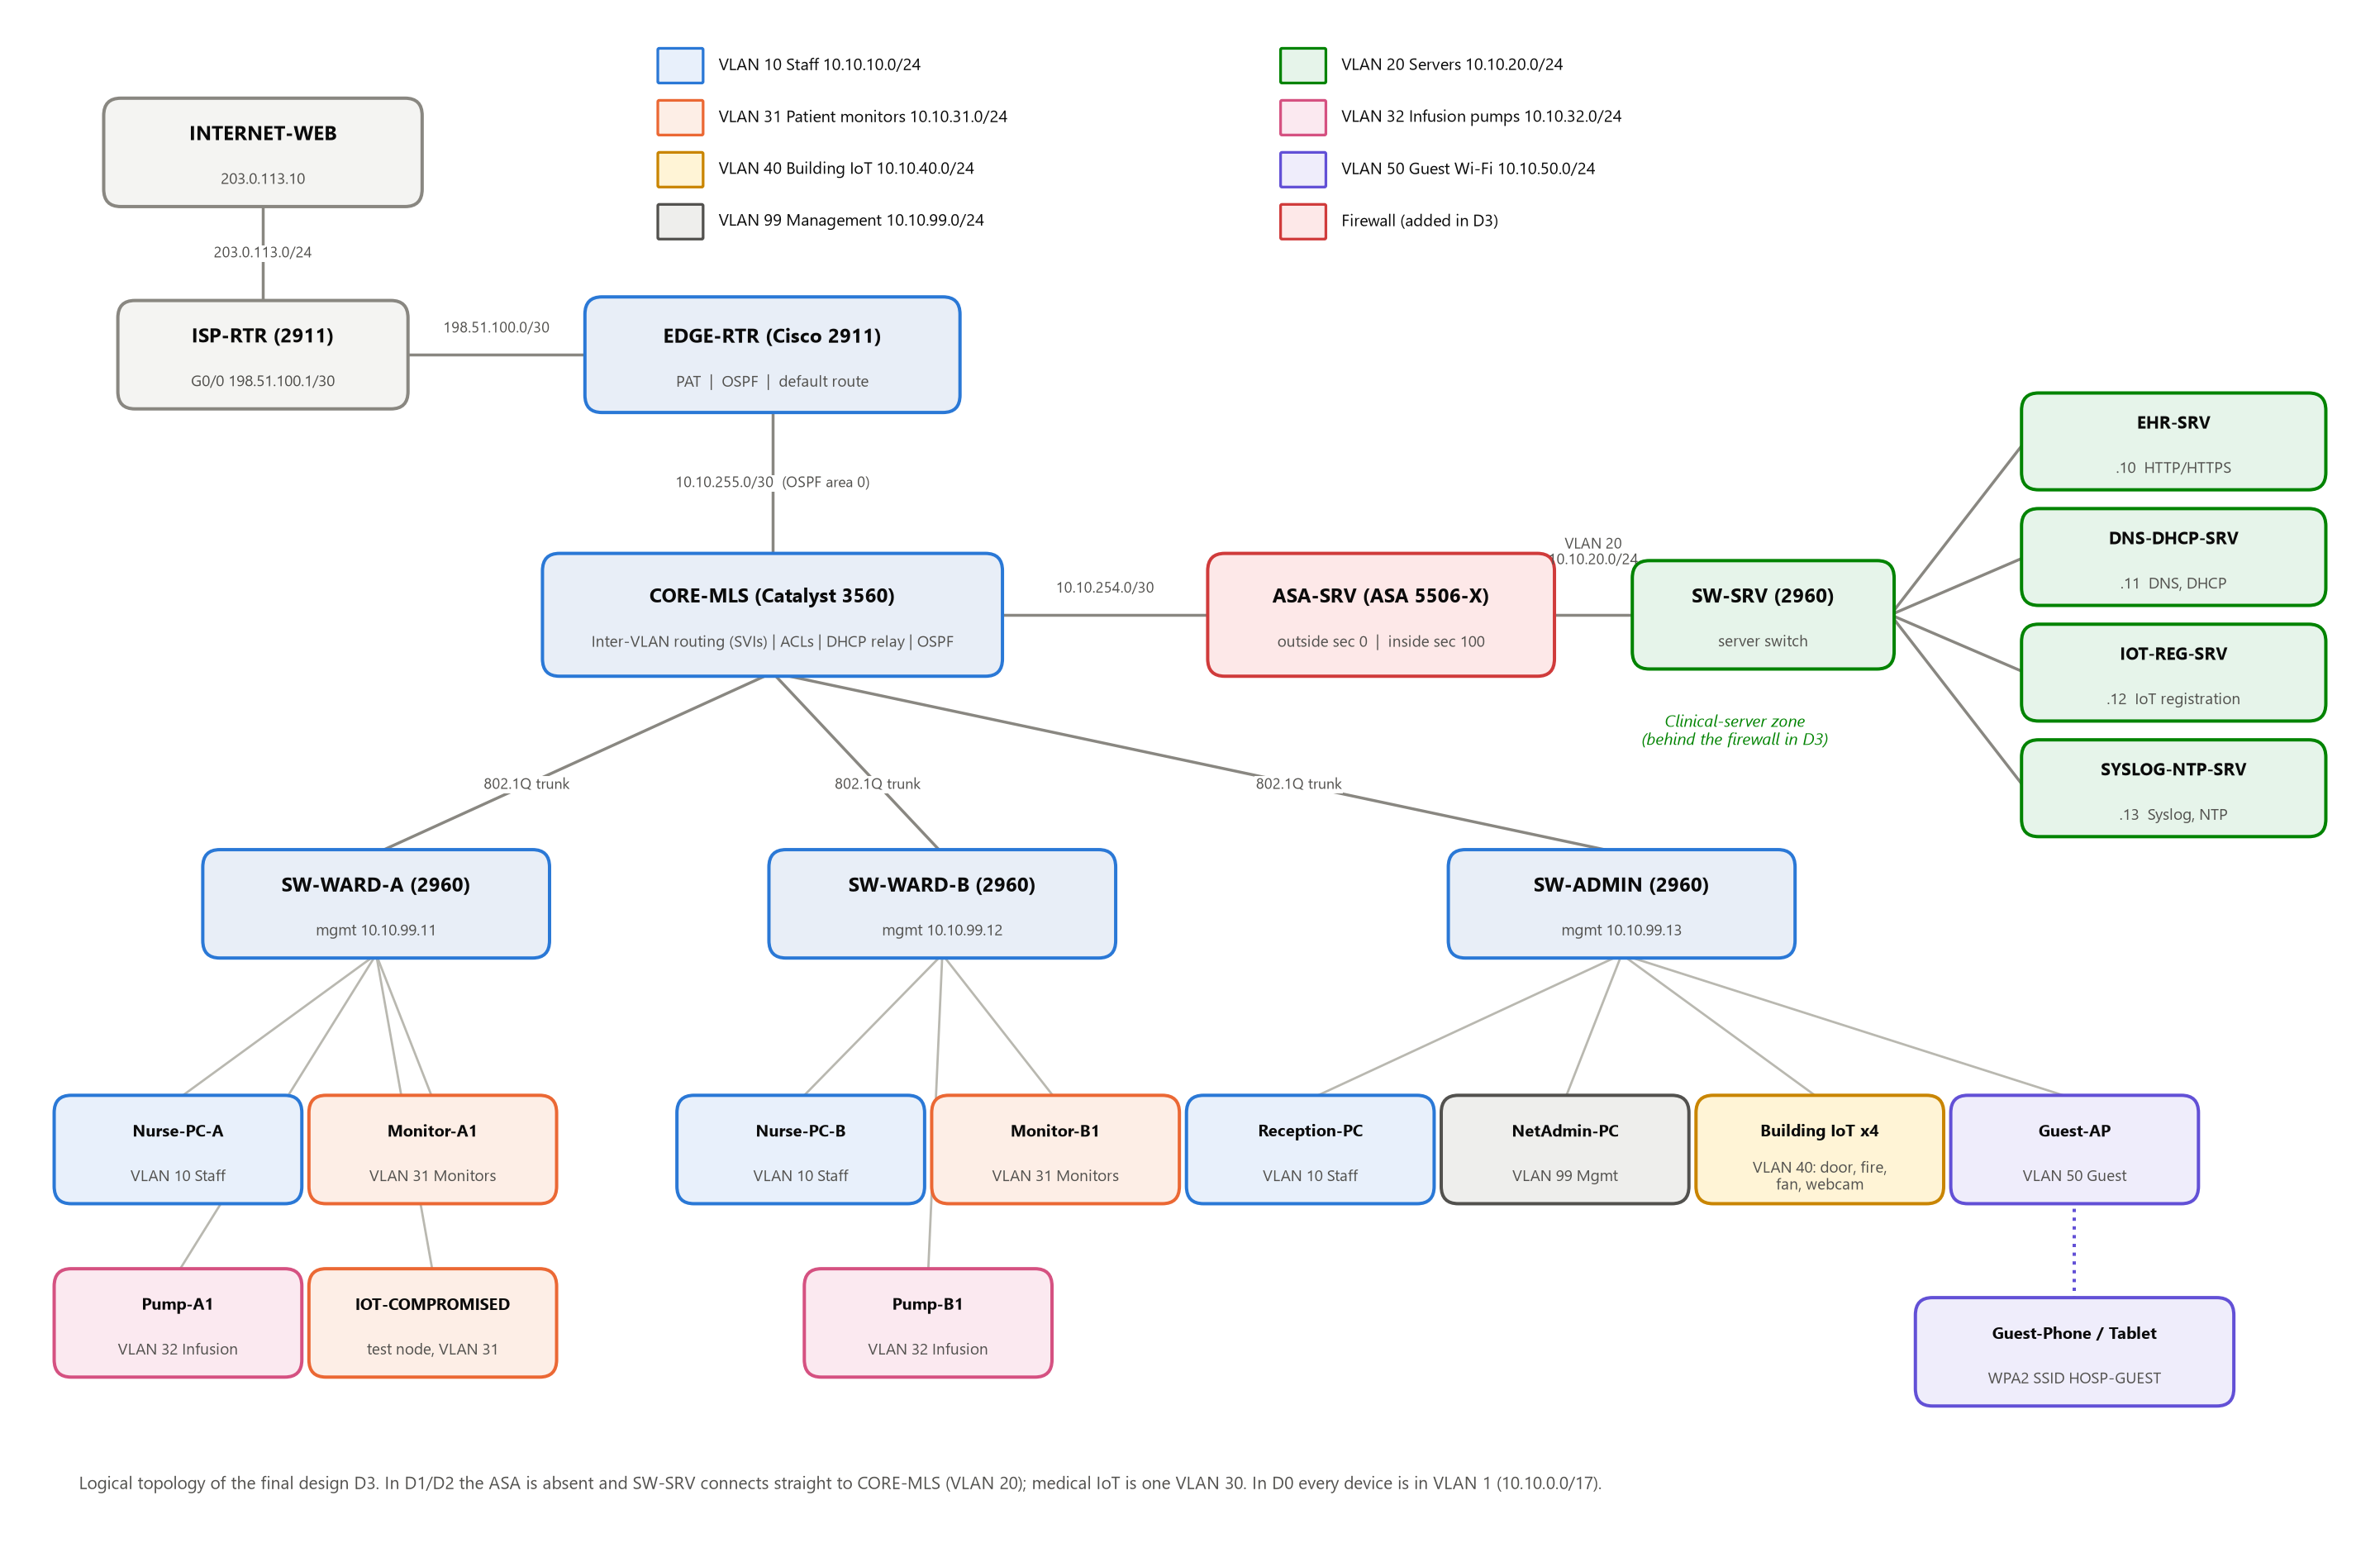
\includegraphics[width=0.88\textwidth]{topology.png}
\caption{Logical topology of D3. In D1/D2 the ASA is absent, SW-SRV attaches to CORE-MLS in VLAN~20 and all medical IoT shares VLAN~30. In D0 every device is in VLAN~1 (10.10.0.0/17). IOT-COMPROMISED is the test node at location L1.}
\label{fig:topology}
\end{figure*}

% AUTO-GENERATED by paper/gen_tables.py -- do not edit by hand; edit the data and re-run.
\begin{table}[t]
\centering
\caption{VLAN and addressing plan extracted from the configurations (10.10.\textit{VLAN}.0/24, gateway .1).}
\label{tab:vlans}
\scriptsize
\setlength{\tabcolsep}{3pt}
\begin{tabular}{@{}rllll@{}}
\toprule
VLAN & Name & Subnet & Designs & Members \\
\midrule
1 & default (flat) & 10.10.0.0/17 & D0 & Every device (flat) \\
10 & STAFF & 10.10.10.0/24 & D1--D3 & Nurse PCs, reception PC \\
20 & SERVERS & 10.10.20.0/24 & D1--D3 & EHR, DNS/DHCP, IoT reg., Syslog/NTP \\
30 & MED-IOT & 10.10.30.0/24 & D1--D2 & All medical IoT \\
31 & MED-MONITORS & 10.10.31.0/24 & D3 & Patient monitors \\
32 & MED-INFUSION & 10.10.32.0/24 & D3 & Infusion pumps \\
40 & BLDG-IOT & 10.10.40.0/24 & D1--D3 & Door, fire monitor, fan, webcam \\
50 & GUEST & 10.10.50.0/24 & D1--D3 & Guest Wi-Fi clients \\
99 & MGMT & 10.10.99.0/24 & D1--D3 & Switch mgmt, NetAdmin-PC \\
998 & NATIVE-UNUSED & -- & D3 & Unused native VLAN on trunks \\
999 & BLACKHOLE & -- & D3 & Parked (shut) ports \\
\bottomrule
\end{tabular}
\end{table}


\subsection{Designs}
\label{sec:designs}
The four designs share devices, cabling, servers and end-device settings. The one exception is that D3 inserts an ASA~5506-X between CORE-MLS and SW-SRV. Otherwise only the device configurations change.

\textbf{D0 Flat:} one broadcast domain (10.10.0.0/17) and Telnet management with a shared password.
\textbf{D1 VLAN-only:} six role VLANs (staff 10, servers 20, medical IoT 30, building IoT 40, guest 50, management 99), routed by CORE-MLS without filtering.
\textbf{D2 Zone ACLs:} D1 plus inbound ACLs on SVIs 30, 40 and 50. IoT may reach the server subnet on any port, and guests may reach only DHCP, DNS and the Internet (Table~\ref{tab:acl}). Staff and management stay unfiltered.
\textbf{D3 Micro-segmentation:} monitors (VLAN~31) and pumps (VLAN~32) are split, and every IoT ACL has one service permit, TCP~80 to the registration server. ICMP echo-replies towards VLAN~99 are also permitted, so administrators can ping devices that cannot start a ping themselves. The server subnet moves behind the ASA. Its \cfg{OUTSIDE-IN} policy (\aceAsaDthree{} ACEs) repeats every permit statefully~\cite{ciscoasa922}; for example, only 10.10.10.0/24 reaches the EHR. Every access port runs sticky port security with \cfg{violation shutdown}, PortFast and BPDU Guard. DHCP snooping trusts only the uplinks~\cite{rfc3046}. Trunks use native VLAN~998, explicit allowed lists and \cfg{nonegotiate}, and unused ports are shut in VLAN~999. Management is SSHv2 only~\cite{rfc4253}, from VLAN~99 only (\cfg{access-class 10 in}).

% AUTO-GENERATED by paper/gen_tables.py -- do not edit by hand; edit the data and re-run.
\begin{table}[t]
\centering
\caption{Key ACL lines, verbatim from the configuration files (``!'' lines added as labels). D2's zone permit admits the whole server subnet, so the F-1 and H-1 denies must carve out router addresses; D3 permits one host and one port.}
\label{tab:acl}
\scriptsize
\begin{minipage}{\columnwidth}
\begin{verbatim}
! D2 CORE-MLS: coarse zone ACL, SVI 30 (inbound)
ip access-list extended MEDIOT-IN
 permit udp any host 255.255.255.255 eq 67
 permit udp any host 10.10.20.11 eq 67
! F-1: exclude the core's own SVI-20 address
 deny ip any host 10.10.20.1
 permit ip 10.10.30.0 0.0.0.255 10.10.20.0 0.0.0.255
 deny ip any any
! D2 GUEST-IN (deny lines only)
! H-1: exclude EDGE-RTR's WAN /30
 deny ip any 198.51.100.0 0.0.0.3
 deny ip any 10.0.0.0 0.255.255.255
! D3 CORE-MLS: least privilege, SVI 31 (inbound)
ip access-list extended MONITORS-IN
 permit udp any host 255.255.255.255 eq 67
 permit udp any host 10.10.20.11 eq 67
 permit tcp 10.10.31.0 0.0.0.255 host 10.10.20.12 eq 80
 permit icmp 10.10.31.0 0.0.0.255 10.10.99.0 0.0.0.255 echo-reply
 deny ip any any
! D3 ASA-SRV access-list OUTSIDE-IN extended (excerpt)
 permit tcp 10.10.10.0 255.255.255.0 host 10.10.20.10 eq 80
 permit tcp 10.10.31.0 255.255.255.0 host 10.10.20.12 eq 80
 deny ip any any
\end{verbatim}
\end{minipage}
\end{table}


\subsection{Pre-deployment verification}
\label{sec:verify}
Before the designs were tested in the simulator, two independent checks reviewed the configurations. The first is a static reachability analyser (\texttt{tools/policy\_analyzer.py}) that reads only the configuration files and the end-device sheet. It models bridge domains, connected, static and OSPF routes, IOS and ASA ACLs with first-match semantics, ASA security levels and connection state, PAT, VTY rules, DHCP relay and snooping, and port security. It walks every test packet hop by hop and records the configuration line that decides it. A pytest suite (125 tests) checks the ACL engine and lints the configurations. It also mutates them, for example by removing an ACL layer or snooping trust, to confirm that a verdict flips. The second check is a third-party configuration-review checklist (ECC~2.2.3 \texttt{network-config-reviewer}), whose findings are recorded in the project's \texttt{tests/FINDINGS.md}. Findings were fixed in the configuration files, and the original files were archived so that both versions can be analysed (Section~\ref{sec:res-verify}).

\subsection{Threat model and test suite}
The adversary fully controls one IoT device and can send arbitrary IP traffic from its port and address. The adversary knows the addressing plan but holds no credentials and cannot exploit IOS or ASA software. Packet Tracer smart devices cannot originate attack traffic, so a laptop (IOT-COMPROMISED) takes the device's port, VLAN and DHCP lease. It is placed at L1, SW-WARD-A Fa0/4 (medical VLAN 30/31); at L2, SW-WARD-B Fa0/4; and at L3, SW-ADMIN Fa0/7 (building VLAN~40). Table~\ref{tab:attackdef} lists the tests and their nearest ATT\&CK techniques~\cite{mitreattack}. A1 probes a fixed inventory of 23 hosts and 10 services. The hosts are staff, servers, IoT, guests and five network-device addresses; the services are EHR HTTP/HTTPS, IoT HTTP, DNS, an Internet web server, and Telnet/SSH on five devices. A1--A4 run at L1--L3 and A5--A8 at fixed ports, three trials each. Nine functional tests (Table~\ref{tab:functional}) check that legitimate flows still work.

\begin{table}[t]
\centering
\caption{Tests and nearest MITRE ATT\&CK techniques.}
\label{tab:attackdef}
\scriptsize
\setlength{\tabcolsep}{2.5pt}
\begin{tabular}{@{}lp{0.56\columnwidth}p{0.30\columnwidth}@{}}
\toprule
ID & Procedure & ATT\&CK \\
\midrule
A1 & ICMP sweep of the 23-host inventory & T1018, T1046 \\
A2 & HTTP to the EHR (10.10.20.10) & T1213 \\
A3 & IoT-server login page; ping Pump-A1 (other class) & T1021 \\
A4 & Telnet/SSH to switch, gateway and router addresses & T1021.004 \\
A5 & Rogue DHCP server on a staff jack (SW-WARD-A Fa0/5) & T1557.003 \\
A6 & Laptop replaces Monitor-A1 on SW-WARD-A Fa0/2 & T1200 \\
A7 & Guest phone: HTTP to the EHR & T1213 \\
A8 & Rogue 2960 on a staff jack negotiates a trunk (DTP) & T1200, T1599 \\
Q1 & Detect node from ACL deny counters; move its port to VLAN~999 & (response) \\
O1 & 10-ping RTT and tracert hops for three legitimate flows & -- \\
\bottomrule
\end{tabular}
\end{table}

\subsection{Automated execution (ptlab)}
The stock Packet Tracer MCP bridge can only exchange ICMP between named devices. Our gateway, ptlab, patches Packet Tracer's script module with a generic evaluation hook (\texttt{ptEval}). On top of it, it adds 16 tools to the 18 stock ones: PC command output (ping, telnet, ssh, nslookup, tracert), a browser client, IOS \cfg{show} capture, and configuration of server services, DHCP pools and DNS records. These are served over a loopback REST API and an MCP proxy. A runner opens each design file and applies the GUI set-up checklist. It then runs A1--A8, Q1, O1 and the automatable functional tests (all except F3 and F8, which stay manual), and writes every observation with raw evidence to the result files. Q1 snapshots the deny counters of the node's SVI ACL while the node pings a management address. After three new denies it locates the node's port in the MAC address table and moves it to VLAN~999. It then records the time to detect and contain, and whether staff can still reach the EHR. Before and after each of A1--A4 the runner reads the CORE-MLS and ASA deny counters; a rise counts as a detection.

\subsection{Metrics}
An attack run is \emph{succeeded} (S) if it reaches every target in scope, \emph{partial} (P) if it reaches some, and \emph{blocked} (B) if it reaches none. Per design we report the majority over runs, with ties going to the outcome worse for the defender. Attack surface counts reachable hosts and services. The metrics follow the literature. Attack-surface reduction is $\mathrm{ASR}=1-\text{reachable}/23$, and the blast radius $\mathrm{BR}_w$ weights each reachable host by an asset-criticality score that we assign (1--5)~\cite{Odule2026SimulationValidation}. Attack block rate (ABR) is the share of blocked attempts. Policy-compliance rate (PCR) counts blocked unauthorised plus passed authorised checks~\cite{Mughaid2026SecureAdaptive}. Detection coverage is the share of attack windows with a deny-counter rise. Fisher's exact test compares blocked attempts between adjacent designs. Configuration cost counts the commands in all device files (excluding comments and mode wrappers), the ACEs, and the 12 security features detected by configuration pattern.

% =====================================================================
\section{Results}
\label{sec:results}
% =====================================================================
% Every table here is generated from ../results/*.csv by gen_tables.py.
% Unmeasured cells are printed as expected values with a visible note.
% TODO(authors): once the Packet Tracer runs are in, re-read the prose of
% this section against the measured tables and add your interpretation of
% any cell where Packet Tracer differs from the prediction.

\ifmeasured\else
\noindent\fbox{\parbox{\dimexpr\columnwidth-2\fboxsep-2\fboxrule}{\footnotesize\textbf{Data status.} Configuration cost (Tables~\ref{tab:fix} and~\ref{tab:complexity}) is measured. Analyser verdicts are computed from the configurations. Attack, surface, functional and metric values are expected outcomes, marked as such, until the Packet Tracer runs are recorded.}}
\par\medskip
\fi

\subsection{Pre-deployment findings}
\label{sec:res-verify}
\ifhavefix
The analyser and the review found three real defects and one inconsistent expectation before any simulator run (Table~\ref{tab:fix}).

\emph{Router-self-address class (F-1, H-1).} In D2, \cfg{MEDIOT-IN} and \cfg{BLDGIOT-IN} permit IoT traffic to 10.10.20.0/24. That subnet contains the core's own SVI-20 address 10.10.20.1, and the core's VTY lines accept Telnet with a shared password and no \cfg{access-class}. A compromised IoT device could therefore log in to CORE-MLS even though every address the test plan probed was denied, so A4 was partial, not blocked. The review then found the mirror image for guests. \cfg{GUEST-IN} denied only 10.0.0.0/8, but EDGE-RTR's WAN address 198.51.100.2 lies outside that range and has the same weak VTY. A guest could open a session on the edge router, and from there on the core. In both cases the ACL names a range and forgets that a router also owns an address in, or just outside, that range. The fixes are one deny each, placed before the zone permit (Table~\ref{tab:acl}). The analyser confirms that both management paths close, and the IoT node's reach in D2 falls from \fixHostsDtwoPre{}/\fixSvcDtwoPre{} to \fixHostsDtwoPost{}/\fixSvcDtwoPost{} hosts/services. D3 was never affected: host-specific permits exclude every gateway address, and VTY access is limited to VLAN~99.

\emph{UDP/67 exfiltration (F-3).} Every SVI ACL in D2 and D3 began with \cfg{permit udp any any eq 67}, so DHCP could work before a client had an address. That line also lets UDP/67 leave through PAT to any Internet host, a one-way channel that survived micro-segmentation. Restricting it to the broadcast address and the DHCP server closes the channel, and all nine functional tests still pass.

\emph{Unhardened server switch (F-4).} The 21 unused SW-SRV ports in D3 were up in VLAN~1 on the firewall's trusted side, and they are now parked and shut. Finally, the A3 expectation for D2 at L3 was corrected to partial. The cross-class target Pump-A1 sits in another VLAN, so \cfg{BLDGIOT-IN} denies it (F-2).

The fixes add \fixDeltaDtwo{} lines (\fixDeltaAcesDtwo{} ACEs) to D2 and \fixDeltaDthree{} (\fixDeltaAcesDthree{}) to D3. With them, the analyser's verdicts disagree with the expected matrix in \fixDisDtwoPost{} of the 15 D2 attack runs, against \fixDisDtwoPre{} before.
\fi

% AUTO-GENERATED by paper/gen_tables.py -- do not edit by hand; edit the data and re-run.
\begin{table}[t]
\centering
\caption{Pre-deployment fixes (F-1, H-1, F-3, F-4) recomputed by the static analyser on the archived pre-fix and the current configurations. Lines and ACEs are counted; the other columns are analyser predictions. A4: verdict at L1/L2/L3; H/S: hosts/services reachable from the IoT node; G$\rightarrow$E: guest can open a management session on EDGE-RTR's WAN address; U67: UDP/67 reaches the Internet; Idle: unused SW-SRV ports left up (F-4 concerns D3 only).}
\label{tab:fix}
\scriptsize
\setlength{\tabcolsep}{3pt}
\begin{tabular}{@{}lccccccc@{}}
\toprule
 & Lines & ACEs & A4 & H/S & G$\rightarrow$E & U67 & Idle \\
\midrule
D2 pre-fix & 293 & 11 & P/P/P & 9/5 & yes & yes & 21 \\
D2 post-fix & 302 & 17 & B/B/B & 8/4 & no & no & 21 \\
\midrule
D3 pre-fix & 559 & 47 & B/B/B & 2.7/1 & no & yes & 21 \\
D3 post-fix & 571 & 52 & B/B/B & 2.7/1 & no & no & 0 \\
\bottomrule
\end{tabular}
\end{table}


\subsection{Functional preservation (RQ2)}
All nine legitimate flows pass in every design (Table~\ref{tab:functional})\expnote; the analyser predicts the same. Each D3 permit was written for one of these flows. F3 and F8 use TCP~80 to 10.10.20.12. F4 uses the DHCP permits. F9 uses the four ASA entries that admit Syslog and NTP only from the two transit /30s. F7 moves from Telnet to SSH but stays available from VLAN~99.

% AUTO-GENERATED by paper/gen_tables.py -- do not edit by hand; edit the data and re-run.
\begin{table}[t]
\centering
\caption{Functional preservation: legitimate flows that must keep working in every design (\cmark~pass, \xmark~fail). \textit{(expected, not yet measured)}}
\label{tab:functional}
\footnotesize
\setlength{\tabcolsep}{4pt}
\begin{tabular}{@{}llcccc@{}}
\toprule
ID & Legitimate flow & D0 & D1 & D2 & D3 \\
\midrule
F1 & Staff PC opens EHR by name (DNS+HTTP) & \cmark & \cmark & \cmark & \cmark \\
F2 & Staff PC pings EHR-SRV & \cmark & \cmark & \cmark & \cmark \\
F3 & All 8 IoT devices on IOT-REG-SRV & \cmark & \cmark & \cmark & \cmark \\
F4 & DHCP lease in the correct subnet & \cmark & \cmark & \cmark & \cmark \\
F5 & Guest phone reaches Internet web & \cmark & \cmark & \cmark & \cmark \\
F6 & Staff Internet access via PAT & \cmark & \cmark & \cmark & \cmark \\
F7 & NetAdmin manages switches (Telnet/SSH) & \cmark & \cmark & \cmark & \cmark \\
F8 & IoT rule: smoke $\rightarrow$ HVAC fan & \cmark & \cmark & \cmark & \cmark \\
F9 & Syslog server receives device logs & \cmark & \cmark & \cmark & \cmark \\
\midrule
\multicolumn{2}{@{}l}{Pass rate} & 9/9 & 9/9 & 9/9 & 9/9 \\
\bottomrule
\end{tabular}
\end{table}


\subsection{Attack outcomes}
Table~\ref{tab:attacks} gives the outcome matrix\expnote. D1 blocks nothing (\succeededDone{} of \nAttacks{} succeed), because CORE-MLS routes between all SVIs. This reproduces the finding of Sifawa et al.~\cite{Sifawa2026ImplementationEvaluation} with an IoMT attacker. D2 blocks infrastructure access (A4, after F-1) and the guest pivot (A7). It does not protect the EHR (A2): \cfg{permit ip} admits the whole server subnet on every port. A5 and A6 are Layer-2 attacks inside one VLAN, which no SVI ACL sees. D3 blocks \blockedDthree{} of \nAttacks{}. \cfg{MONITORS-IN} has no entry for the EHR, and the ASA admits the EHR only from staff. DHCP snooping drops the rogue server's OFFER on the untrusted Fa0/5, and the sticky MAC on Fa0/2 err-disables the port when the laptop appears. A1 and A3 stay partial by construction. Same-VLAN peers answer at Layer~2 without crossing an SVI, and TCP~80 to the registration server must stay open. The rogue switch (A8) forms a trunk only in D0, whose ports are dynamic; access-mode ports refuse DTP, and in D3 BPDU Guard also err-disables the port. Q1 can act only where an SVI ACL produces deny counters, that is in D2 and D3\ifhaveqone, with a mean time to contain of \qOneContain~s\fi.

% AUTO-GENERATED by paper/gen_tables.py -- do not edit by hand; edit the data and re-run.
\begin{table}[t]
\centering
\caption{Attack outcome per design (majority vote over all locations $\times$ trials; ties go to the worse outcome). \oS{}~succeeded, \oP{}~partial, \oB{}~blocked; for Q1, \oB{} means the node was detected and quarantined. \textit{(expected, not yet measured)}}
\label{tab:attacks}
\footnotesize
\setlength{\tabcolsep}{4pt}
\begin{tabular}{@{}llcccc@{}}
\toprule
ID & Attack & D0 & D1 & D2 & D3 \\
\midrule
A1 & Recon ping sweep & \oS & \oS & \oP & \oP \\
A2 & EHR access (HTTP) & \oS & \oS & \oS & \oB \\
A3 & IoT-server / cross-class & \oS & \oS & \oS & \oP \\
A4 & Telnet/SSH to infra & \oS & \oS & \oB & \oB \\
A5 & Rogue DHCP server & \oS & \oS & \oS & \oB \\
A6 & Unauthorised device & \oS & \oS & \oS & \oB \\
A7 & Guest $\rightarrow$ EHR pivot & \oS & \oS & \oB & \oB \\
\midrule
A8 & Rogue switch (DTP) & \oS & \oB & \oB & \oB \\
Q1 & Auto-quarantine & \oS & \oS & \oB & \oB \\
\bottomrule
\end{tabular}
\end{table}


\subsection{Attack surface and derived metrics (RQ1)}
Reachable hosts fall from \hostsPctDzero\% (D0, D1) to \hostsPctDtwo\% (D2) and \hostsPctDthree\% (D3), and reachable services from \svcPctDzero\% to \svcPctDtwo\% and \svcPctDthree\% (Table~\ref{tab:surface})\expnote. In D2 the reachable hosts are the four servers and four same-VLAN IoT peers. In D3 they are only same-VLAN peers: two monitors from L1 and L2, four building devices from L3. Location matters only in D3, which is the source of its standard deviation; Packet Tracer outcomes do not vary between trials.
\ifhavemetrics
Weighting reachable hosts by criticality makes the step from D2 to D3 larger. $\mathrm{BR}_w$ falls from \brwDzero{} to \brwDtwo{} and \brwDthree{} (Table~\ref{tab:metrics}), because D2 still exposes the EHR and, from the wards, both pumps. Blocked attempts differ significantly between D1 and D2 ($p=\fisherDtwo$) and between D2 and D3 ($p=\fisherDthree$)\expnote.
\fi

% AUTO-GENERATED by paper/gen_tables.py -- do not edit by hand; edit the data and re-run.
\begin{table}[t]
\centering
\caption{Attack surface reachable from the compromised node: hosts answering (of 23) and services accepting a connection (of 10); per-location means and overall mean$\pm$sd over 3 locations $\times$ trials. \textit{(expected, not yet measured)}}
\label{tab:surface}
\scriptsize
\setlength{\tabcolsep}{3pt}
\begin{tabular}{@{}lrrrrrrr@{}}
\toprule
& \multicolumn{5}{c}{Hosts reachable} & \multicolumn{2}{c}{Services} \\
\cmidrule(lr){2-6}\cmidrule(l){7-8}
Design & L1 & L2 & L3 & mean$\pm$sd & \% & mean$\pm$sd & \% \\
\midrule
D0 Flat & 23 & 23 & 23 & 23.00$\pm$0.00 & 100 & 10.00$\pm$0.00 & 100 \\
D1 VLAN-only & 23 & 23 & 23 & 23.00$\pm$0.00 & 100 & 10.00$\pm$0.00 & 100 \\
D2 Zone ACL & 8 & 8 & 8 & 8.00$\pm$0.00 & 35 & 4.00$\pm$0.00 & 40 \\
D3 Micro-seg & 2 & 2 & 4 & 2.67$\pm$1.00 & 12 & 1.00$\pm$0.00 & 10 \\
\bottomrule
\end{tabular}
\par\vspace{2pt}\parbox{\columnwidth}{\scriptsize L1 = L1-WardA-MedIoT; L2 = L2-WardB-MedIoT; L3 = L3-BuildingIoT. sd is the sample standard deviation over all runs of a design, so it mixes location and trial variation.}
\end{table}

\ifhavemetrics% AUTO-GENERATED by paper/gen_tables.py -- do not edit by hand; edit the data and re-run.
\begin{table}[t]
\centering
\caption{Derived security metrics (tools/metrics.py): attack-surface reduction (ASR), criticality-weighted blast radius (BR$_w$), attack block rate (ABR), policy-compliance rate (PCR), detection coverage (DET) and Fisher's exact $p$ for blocked attempts against the previous design. \textit{(expected, not yet measured)}}
\label{tab:metrics}
\footnotesize
\setlength{\tabcolsep}{4pt}
\begin{tabular}{@{}lcccccc@{}}
\toprule
Design & ASR & BR$_w$ & ABR & PCR & DET & $p$ vs prev. \\
\midrule
D0 Flat & 0.00 & 1.00 & 0.00 & 0.17 & -- & -- \\
D1 VLAN-only & 0.00 & 1.00 & 0.00 & 0.17 & -- & 1 \\
D2 Zone ACL & 0.65 & 0.39 & 0.27 & 0.39 & -- & 2.1e-04 \\
D3 Micro-seg & 0.88 & 0.12 & 0.60 & 0.67 & -- & 0.0027 \\
\bottomrule
\end{tabular}
\par\vspace{2pt}\parbox{\columnwidth}{\scriptsize BR$_w$ weights each reachable host by an asset-criticality score (1--5) assigned by the authors (EHR and pumps 5; infrastructure and monitors 4). Packet Tracer outcomes are deterministic, so $p$ reflects the number of attempts, not run-to-run noise.}
\end{table}
\fi

\subsection{Configuration cost and overhead (RQ3)}
Configuration grows from \cfgLinesDzero{} lines in D0 to \cfgLinesDone{}, \cfgLinesDtwo{} and \cfgLinesDthree{} ($\times$\lineRatioDthree{}), and ACEs from \acesDzero{} to \acesDone{}, \acesDtwo{} and \acesDthree{} (Table~\ref{tab:complexity}). The steps are uneven. D0$\rightarrow$D1 costs \deltaLinesDone{} lines and no ACEs, D1$\rightarrow$D2 \deltaLinesDtwo{} lines on one device, and D2$\rightarrow$D3 \deltaLinesDthree{} lines across six existing devices and the new ASA. Of D3's \acesDthree{} ACEs, \aceCoreDthree{} sit on the core SVIs, \aceAsaDthree{} on the ASA and \aceStdDthree{} in the standard VTY and NAT lists. Fig.~\ref{fig:tradeoff} plots attacks blocked against lines. The curve is flat from D0 to D1 and steepest from D1 to D2. On the legitimate path, D3 adds one Layer-3 device (the ASA) and one policy evaluation between staff and the EHR (Appendix Table~\ref{tab:overhead}). \ifhaveoverhead The measured RTT and hop counts are given there. \else The RTT and hop-count test O1 has not yet been run. \fi

% AUTO-GENERATED by paper/gen_tables.py -- do not edit by hand; edit the data and re-run.
\begin{table}[t]
\centering
\caption{Configuration complexity per design, counted from the device configuration files (comments and mode-change wrappers excluded).}
\label{tab:complexity}
\footnotesize
\begin{tabular}{@{}lrrrr@{}}
\toprule
Design & Devices & Config lines & ACEs & Sec.\ features \\
\midrule
D0 Flat & 7 & 189 ($\times$1.00) & 1 & 0 \\
D1 VLAN-only & 7 & 274 ($\times$1.45) & 1 & 1 \\
D2 Zone ACL & 7 & 302 ($\times$1.60) & 17 & 2 \\
D3 Micro-seg & 8 & 571 ($\times$3.02) & 52 & 12 \\
\bottomrule
\end{tabular}
\end{table}


\begin{figure}[t]
\centering
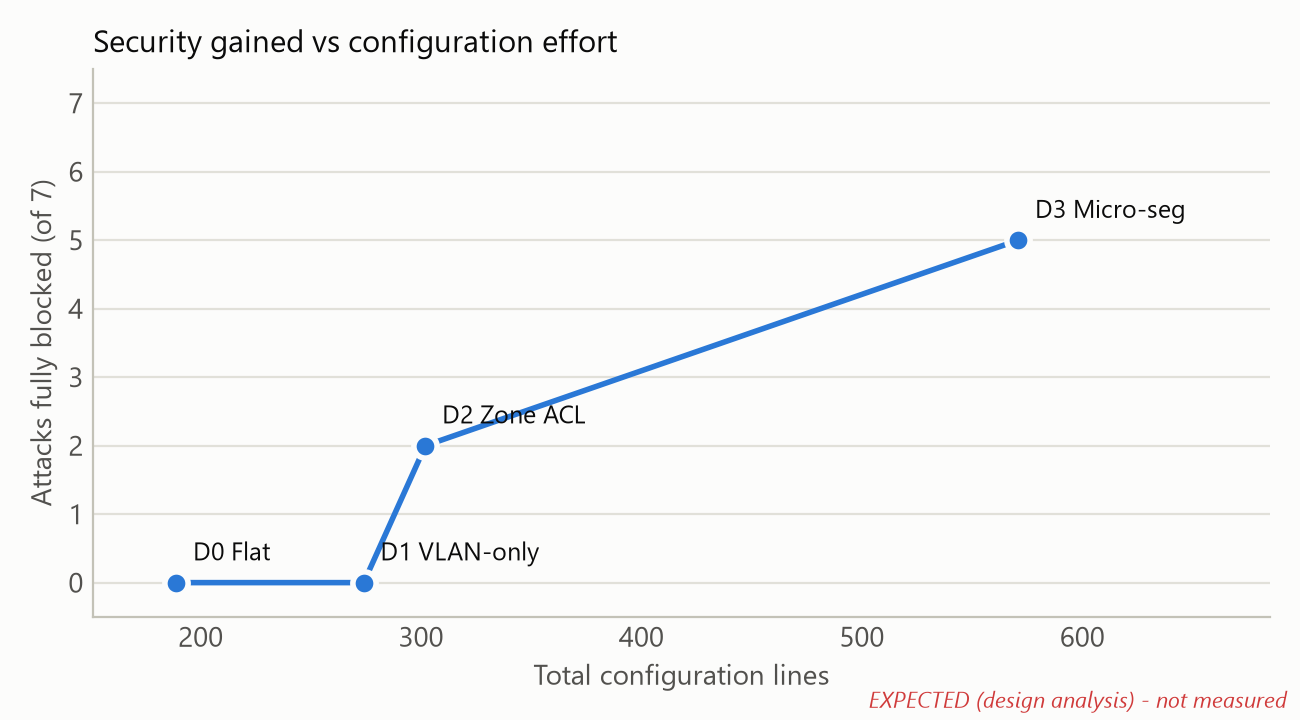
\includegraphics[width=\columnwidth]{tradeoff.png}
\caption{Core attacks fully blocked (of 7) versus total configuration lines per design.\expnote}
\label{fig:tradeoff}
\end{figure}

% =====================================================================
\section{Discussion}
\label{sec:discussion}
% =====================================================================
% TODO(authors): add your own interpretation once the measured data is in,
% in particular whether the observed matrix changes any argument below.

\textbf{VLANs enable policy; they are not policy.}
D1 costs \deltaLinesDone{} lines and contains nothing, but it creates the subnets and SVIs on which every later rule is applied. Once VLANs exist, D2's first protection costs \deltaAcesDtwo{} ACEs on one device. The number of VLANs says little about containment; what each SVI may forward says almost everything.

\textbf{Zone rules must exclude the network's own addresses.}
The router-self-address class is easy to miss because the ACL reads correctly. ``IoT may reach the server zone'' and ``guests may not reach 10/8'' both describe hosts, while routers also own addresses inside and outside those ranges. A test plan written from the same mental model misses the exposure too: our A4 procedure probed the management VLAN, the node's own gateway and the core--edge link, never 10.10.20.1. A reachability model that enumerates every interface address of every device found the gap. In practice this argues for pairing any zone policy with a VTY \cfg{access-class} and with an explicit deny for infrastructure addresses ahead of the zone permit. D3 reaches the same effect another way: an \cfg{access-class}, host-specific permits that never match a gateway, and a server gateway that sits on the ASA.

\textbf{Least privilege is what protects data.}
D2 cuts reachable services from 10 to 4 but leaves the EHR open, because the most sensitive asset and the service every IoT device needs share one zone. Only a host-and-port rule separates them, which is the practical meaning of a per-resource access decision~\cite{nist80027}. The analyser's mutation tests show that the core ACLs and the ASA each block the EHR alone. The firewall therefore adds independence and connection state rather than a new outcome in Table~\ref{tab:attacks}, at the price of \aceAsaDthree{} ACEs that must be kept consistent with the core by hand.

\textbf{Minimum viable segmentation.}
The step from D2 to D3 bundles independent controls, and each D3 block has a single cause. Host-and-port SVI ACLs close A2 and the cross-class part of A3, DHCP snooping closes A5, and port security closes A6. For a small hospital without a firewall team we therefore recommend four measures:
(i) D2's zones;
(ii) each IoT zone permit replaced by \cfg{permit tcp \ldots{} host 10.10.20.12 eq 80};
(iii) DHCP snooping and sticky port security on clinical ports;
(iv) SSH with a VTY \cfg{access-class}.
Every line of this set already exists in our D3 files. We have not, however, measured it as a separate design.

\textbf{Complexity is concentrated.}
Most of D3's extra lines are templated Layer-2 hardening: six port-security and STP lines per access port, plus trunk and parking blocks. The policy itself is \aceCoreDthree{}~ACEs on the core and \aceAsaDthree{} on the ASA. The hard part to keep correct is therefore small, and as F-1 and H-1 show, it is exactly where errors hide. This supports running a reachability check on every policy change, rather than relying on hand-written test plans alone.

% =====================================================================
\section{Limitations and Residual Risks}
\label{sec:limits}
% =====================================================================

\textbf{Simulator and attacker.} Packet Tracer~\cite{packettracer} implements a subset of IOS and ASA behaviour. It has no exploit tools, and its end devices cannot craft frames, so double tagging, ARP spoofing and DHCP starvation cannot be tested. Timing is approximate and throughput cannot be measured. A laptop stands in for the compromised device: it is equivalent at the network layer, but it does not model a compromise of the medical application. The analyser assumes, and the live runs must confirm, that inbound SVI ACLs also filter traffic addressed to the switch itself and that IoT registration uses TCP~80.

\textbf{Scope.} The testbed has one site, 23 target hosts and one attacker at a time. Absolute percentages therefore do not carry over to a large hospital; the ordering of the designs is the result we expect to generalise. A1 counts hosts by ICMP, so a host that serves TCP but drops ICMP, such as the registration server in D3, appears only in the service count. \ifmeasured\else The attack, surface, functional and metric values are expected outcomes until the Packet Tracer runs are recorded.\fi

\textbf{Residual risks in D3.} Beyond the fixed defects, the configuration review recorded five open risks (\texttt{tests/FINDINGS.md}, ``ECC network-config-reviewer pass''):
(a) Same-VLAN traffic: two monitors in VLAN~31 still reach each other at Layer~2. This is the source of D3's partial A1 and A3.
(b) H-2: the registration server, the one server every IoT class may reach, shares the ASA's inside segment with the EHR. An exploit of that server would land one hop from patient records.
(c) M-1: the EHR also listens on TCP~80, and IoT registration is HTTP only, so health data can cross the network in cleartext.
(d) M-2: deny ACEs carry no \cfg{log} keyword, and the access switches send no Syslog. Port-security and BPDU Guard events therefore never reach the Syslog server; Q1 relies on ACL counters instead.
(e) M-3: without Dynamic ARP Inspection, a device can spoof its VLAN's gateway.

% =====================================================================
\section{Conclusion and Future Work}
\label{sec:conclusion}
% =====================================================================
We compared four segmentation levels of one smart-hospital network, changing only the security policy, against attacks launched from a compromised IoMT device. \ifmeasured The measurements show \else Configuration analysis predicts\expnote{} \fi that VLANs alone contain nothing and that zone ACLs protect the infrastructure but not the EHR. Only host-and-port least privilege, combined with DHCP snooping and port security, keeps the device away from patient records, and it does so while all nine clinical and IoT flows keep working. Protection costs \cfgLinesDzero{}$\rightarrow$\cfgLinesDthree{} lines and \acesDzero{}$\rightarrow$\acesDthree{} ACEs, most of it templated Layer-2 hardening. Before deployment, an independent reachability analyser and a configuration review caught a router-self-address error that our own test plan would have missed. That error is cheap to fix and easy to repeat.

Future work follows from the residual risks:
(i) isolating same-class devices with private VLANs~\cite{rfc5517}, whose own attack surface must also be assessed~\cite{Alvarez2023PerformanceAnalysis}; Packet Tracer support for PVLAN-edge ports is \probeProtected{};
(ii) device identity through IEEE~802.1X~\cite{ieee8021x} and profile-based network access control~\cite{Garciateodoro2022NovelZero,Allouzi2024EnablingZero};
(iii) Dynamic ARP Inspection and IP Source Guard, built on the DHCP-snooping bindings D3 already keeps;
(iv) a DMZ interface on the ASA for the IoT registration server, an HTTPS-only EHR, and logged denies with switch Syslog;
(v) turning the Q1 loop into controller-driven dynamic segmentation~\cite{Raval2026ImplementationDynamic,Grammatikis2021ModelingDetecting};
(vi) repeating the study on physical switches.
% TODO(authors): add a closing sentence in your own words (e.g. what you
% would tell a hospital IT team), and an acknowledgment if the venue allows.


% Secondary tables (outside the main-text page budget). IEEE order:
% appendices, then the Acknowledgment, then the References.
% =====================================================================
% Appendix: secondary tables (outside the main-text page budget)
% =====================================================================
\appendices
\section{Supplementary tables}
\label{app:tables}
Table~\ref{tab:addressing} lists the routed and management addresses of D3, and Table~\ref{tab:aclinv} shows where each design's ACEs sit. \ifhavestatic Table~\ref{tab:static} gives the analyser's verdict for every attack after the fixes of Section~\ref{sec:res-verify}, and Table~\ref{tab:staticsurface} its reachability counts. \fi Table~\ref{tab:overhead} reports the path analysis and the O1 overhead test\ifhavedetection, and Table~\ref{tab:detection} the detection coverage per attack\fi.

% AUTO-GENERATED by paper/gen_tables.py -- do not edit by hand; edit the data and re-run.
\begin{table}[t]
\centering
\caption{Routed, transit and management addresses in D3 (from the configurations) and server hosts (from the end-device sheet).}
\label{tab:addressing}
\scriptsize
\setlength{\tabcolsep}{3pt}
\begin{tabular}{@{}lllp{0.38\columnwidth}@{}}
\toprule
Device & Intf./port & Address & Role \\
\midrule
ASA-SRV & G1/1 & 10.10.254.2/30 & ASA outside, security-level 0 \\
ASA-SRV & G1/2 & 10.10.20.1/24 & ASA inside, security-level 100 \\
CORE-MLS & G0/1 & 10.10.255.2/30 & Routed link to EDGE-RTR G0/1 \\
CORE-MLS & G0/2 & 10.10.254.1/30 & Routed link to ASA-SRV G1/1 (outside) \\
CORE-MLS & Vlan99 & 10.10.99.1/24 & MANAGEMENT gateway (trusted) \\
EDGE-RTR & G0/0 & 198.51.100.2/30 & WAN to ISP-RTR G0/0 \\
EDGE-RTR & G0/1 & 10.10.255.1/30 & Routed link to CORE-MLS G0/1 \\
ISP-RTR & G0/0 & 198.51.100.1/30 & WAN link to hospital EDGE-RTR G0/0 \\
ISP-RTR & G0/1 & 203.0.113.1/24 & ``Internet'' LAN with public web server \\
SW-ADMIN & Vlan99 & 10.10.99.13/24 & Management \\
SW-WARD-A & Vlan99 & 10.10.99.11/24 & Management \\
SW-WARD-B & Vlan99 & 10.10.99.12/24 & Management \\
EHR-SRV & Fa0/1 & 10.10.20.10/24 & server host \\
DNS-DHCP-SRV & Fa0/2 & 10.10.20.11/24 & server host \\
IOT-REG-SRV & Fa0/3 & 10.10.20.12/24 & server host \\
SYSLOG-NTP-SRV & Fa0/4 & 10.10.20.13/24 & server host \\
INTERNET-WEB & ISP-RTR G0/1 & 203.0.113.10/24 & server host \\
\bottomrule
\end{tabular}
\end{table}

% AUTO-GENERATED by paper/gen_tables.py -- do not edit by hand; edit the data and re-run.
\begin{table}[t]
\centering
\caption{Where the ACEs are: access-control entries per ACL and design (standard ACL~1 selects NAT traffic on EDGE-RTR; standard ACL~10 restricts VTY access).}
\label{tab:aclinv}
\scriptsize
\begin{tabular}{@{}lp{0.70\columnwidth}r@{}}
\toprule
Design & ACL (device): ACEs & Total \\
\midrule
D0 & ACL 1 (1 dev.): 1 & 1 \\
D1 & ACL 1 (1 dev.): 1 & 1 \\
D2 & MEDIOT-IN (CORE-MLS): 5; BLDGIOT-IN (CORE-MLS): 5; GUEST-IN (CORE-MLS): 6; ACL 1 (1 dev.): 1 & 17 \\
D3 & OUTSIDE-IN (ASA-SRV): 16; STAFF-IN (CORE-MLS): 10; MONITORS-IN (CORE-MLS): 5; INFUSION-IN (CORE-MLS): 5; BLDGIOT-IN (CORE-MLS): 5; GUEST-IN (CORE-MLS): 5; ACL 10 (5 dev.): 5; ACL 1 (1 dev.): 1 & 52 \\
\bottomrule
\end{tabular}
\end{table}

\ifhavestatic% AUTO-GENERATED by paper/gen_tables.py -- do not edit by hand; edit the data and re-run.
\begin{table}[t]
\centering
\caption{Static analysis: attack verdicts predicted from the configurations (majority over locations). A star marks a verdict that differs from the design-analysis expectation in Table~\ref{tab:attacks}; the expected value is in parentheses. Computed from the configuration files by a static reachability analyser (\texttt{tools/policy\_analyzer.py}); this is \emph{not} a Packet Tracer measurement.}
\label{tab:static}
\footnotesize
\begin{tabular}{@{}llcccc@{}}
\toprule
ID & Attack & D0 & D1 & D2 & D3 \\
\midrule
A1 & Recon ping sweep & \oS & \oS & \oP & \oP \\
A2 & EHR access (HTTP) & \oS & \oS & \oS & \oB \\
A3 & IoT-server / cross-class & \oS & \oS & \oS & \oP \\
A4 & Telnet/SSH to infra & \oS & \oS & \oB & \oB \\
A5 & Rogue DHCP server & \oS & \oS & \oS & \oB \\
A6 & Unauthorised device & \oS & \oS & \oS & \oB \\
A7 & Guest $\rightarrow$ EHR pivot & \oS & \oS & \oB & \oB \\
\bottomrule
\end{tabular}
\end{table}

\begin{table}[t]
\centering
\caption{Static analysis: hosts and services reachable from the compromised node, mean over locations. ``Any address'' also counts a device reached through any of its interface addresses; ``listed'' counts only the addresses in the test plan. Computed from the configuration files by a static reachability analyser (\texttt{tools/policy\_analyzer.py}); this is \emph{not} a Packet Tracer measurement.}
\label{tab:staticsurface}
\footnotesize
\begin{tabular}{@{}lcccc@{}}
\toprule
& \multicolumn{2}{c}{Hosts} & \multicolumn{2}{c}{Services} \\
\cmidrule(lr){2-3}\cmidrule(l){4-5}
Design & any addr. & listed & any addr. & listed \\
\midrule
D0 Flat & 23 & 23 & 10 & 10 \\
D1 VLAN-only & 23 & 23 & 10 & 10 \\
D2 Zone ACL & 8 & 8 & 4 & 4 \\
D3 Micro-seg & 2.7 & 2.7 & 1 & 1 \\
\bottomrule
\end{tabular}
\end{table}
\fi
% AUTO-GENERATED by paper/gen_tables.py -- do not edit by hand; edit the data and re-run.
\begin{table}[t]
\centering
\caption{Overhead on legitimate traffic. Top: path analysis from topology and configuration. Bottom: test O1, mean ping RTT (10 pings) and tracert hop count \textit{(not yet measured)}.}
\label{tab:overhead}
\scriptsize
\setlength{\tabcolsep}{3pt}
\begin{tabular}{@{}lcccc@{}}
\toprule
Flow / quantity & D0 & D1 & D2 & D3 \\
\midrule
Staff$\rightarrow$EHR: L3 devices in path & 0 & 1 & 1 & 2 \\
Staff$\rightarrow$EHR: policy checks & 0 & 0 & 0 & 2 \\
Monitor$\rightarrow$IoT srv: policy checks & 0 & 0 & 1 & 2 \\
\midrule
Staff$\rightarrow$EHR: RTT (ms) & n.m. & n.m. & n.m. & n.m. \\
Staff$\rightarrow$EHR: hops & n.m. & n.m. & n.m. & n.m. \\
Staff$\rightarrow$Internet: RTT (ms) & n.m. & n.m. & n.m. & n.m. \\
Staff$\rightarrow$Internet: hops & n.m. & n.m. & n.m. & n.m. \\
Admin$\rightarrow$SW-WARD-A: RTT (ms) & n.m. & n.m. & n.m. & n.m. \\
Admin$\rightarrow$SW-WARD-A: hops & n.m. & n.m. & n.m. & n.m. \\
\bottomrule
\end{tabular}
\par\vspace{2pt}\parbox{\columnwidth}{\scriptsize n.m.\ = not yet measured (results/overhead.csv is empty).}
\end{table}

\ifhavedetection% AUTO-GENERATED by paper/gen_tables.py -- do not edit by hand; edit the data and re-run.
% results/detection.csv missing or empty (not yet measured)
\fi


% Template component head "Acknowledgment" (unnumbered, before the references).
% TODO(authors): uncomment and write it, or delete it. Sponsors go in the
% \thanks footnote of the title instead.
% \section*{Acknowledgment}
% ...

\balance
\bibliographystyle{IEEEtran}
\bibliography{refs}

\end{document}
